\documentclass{ximera}[font=12pt]

\title{Subtracting Integers:  Introduction}   % Use xmlatex all -s to compile when SERVE refuses to work.
\author{Kelly Stady}
\license{CC: 0}         % replace with an appropriate license, or set it in xmPreamble

\begin{document}

\begin{abstract}

\end{abstract}

\maketitle
\label{xim:SubtractIntActivity}


\section*{Introduction}

\textbf{Elevation} is the height of a point on earth \textbf{above} ($+$) or \textbf{below} ($-$) sea level.  In geology, the \textbf{elevation span or topographic relief} of a region is the difference between its highest and lowest elevations. Regions with large spans are typically rugged, with high mountain ranges and deep valleys, whereas regions with small spans are generally flatter and more uniform.
\[ \textbf{Elevation Span} = \textrm{Highest Elevation} - \textrm{Lowest Elevation} \]

By calculating the difference between the highest and lowest elevations, geologists can determine if a region is being built up by internal forces (large span) or worn away by the elements (small span).

When both points of interest are above sea level, finding the span is easy.  In Ohio, for example, the highest point (Campbell Hill) is 1,550 feet \textbf{above} sea level, and the lowest point (Ohio River) is 455 feet \textbf{above} sea level, so the elevation span of Ohio is
\[ 1,550 - 455 = 1,095 \ \textrm{feet}. \]

When one elevation is below sea level, finding the span isn't as straightforward.  For instance, in the United States, the highest peak is 20,310 feet \textbf{above} sea level in Denali, Alaska and the lowest basin is 282 feet \textbf{below} sea level in Death Valley, California.  So, the elevation span of the U.S. is given by
\[ 20,310 - (-282). \]

However, from the diagram below, you can see that the span of the U.S. can be found by \emph{adding}.
\[ 20,310 + 282 = 20,592 \ \textrm{feet} \]


\begin{center}
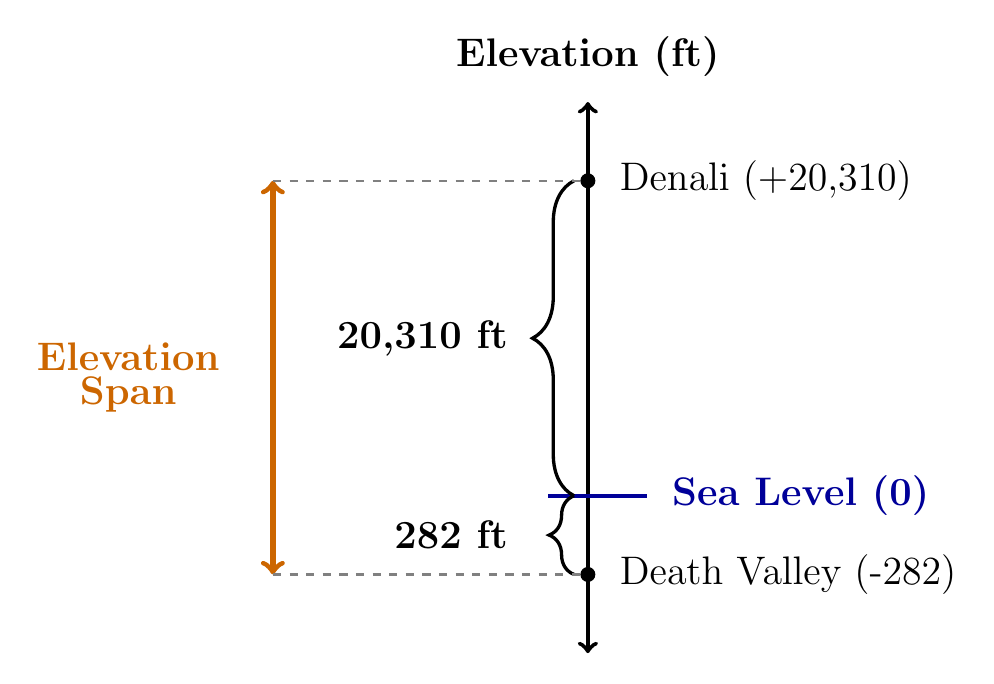
\begin{tikzpicture}[scale=0.5]   %USA Elevation Span
    % Draw Vertical Axis
    \draw[ultra thick, <->] (0,-4) -- (0,10) node[above, yshift=5pt] {\Large\textbf{Elevation (ft)}};

    % Sea Level Line
    \draw[blue!60!black, ultra thick] (-1,0) -- (1.5,0) node[right, xshift=5pt] {\Large\textbf{Sea Level (0)}};

    % Denali Point (+20,310)
    \filldraw[black] (0,8) circle (5pt) node[right, xshift=8pt] {\Large Denali (+20,310)};

    % Death Valley Point (-282)
    \filldraw[black] (0,-2) circle (5pt) node[right, xshift=8pt] {\Large Death Valley (-282)};

    % Braces - Using 'very thick' for the curly lines
    \draw [decorate, decoration={brace, amplitude=9pt, raise=5pt}, very thick] (0,-2) -- (0,0)
        node [midway, left=25pt] {\Large\textbf{282 ft}};

    \draw [decorate, decoration={brace, amplitude=15pt, raise=5pt}, very thick] (0,0) -- (0,8)
        node [midway, left=25pt] {\Large\textbf{20,310 ft}};

    % Total Span Arrow - Two lines, Bold, No Italics
    \draw[<->, orange!80!black, line width=2pt] (-8,-2) -- (-8,8)
        node [midway, left=15pt, align=center] {
            \Large\textbf{Elevation}\\
            \Large\textbf{Span}
        };

    % Guides
    \draw[dashed, gray, thick] (-8,8) -- (0,8);
    \draw[dashed, gray, thick] (-8,-2) -- (0,-2);
\end{tikzpicture}
\end{center}


%Has old data 20,320 instead of 20,310 for Denali
%\emph{Source:} Elevation data provided by the U.S. Geological Survey (USGS), Highest and Lowest Elevations table. Available at %\href{https://www.usgs.gov/educational-resources/highest-and-lowest-elevations}{\textcolor{darkraspberry}{\textbf{usgs.gov}}}.


\normalsize
Although it seems paradoxical, this illustrates a key concept: \textbf{subtracting a number is the same as adding its opposite}.

\[ 20,310 - (-282) =  20,310 + 282 \]



\begin{problem}
China has the largest elevation span in the world. Its highest elevation is 29,032 feet \textbf{above} sea level on Mount Everest and its lowest elevation is
505 feet \textbf{below} sea level at Ayding Lake.

Write the subtraction problem to find China's elevation span.

\begin{multipleChoice}
\choice{$29,032 - 505 $}
\choice{$-29,032 - (-505)$}
\choice[correct]{$29,032 - (-505)$}
\choice{$-29,032 - 505$}
\end{multipleChoice}


\begin{problem}
Use the diagram below to write the subtraction problem as an equivalent addition problem.

\begin{center}
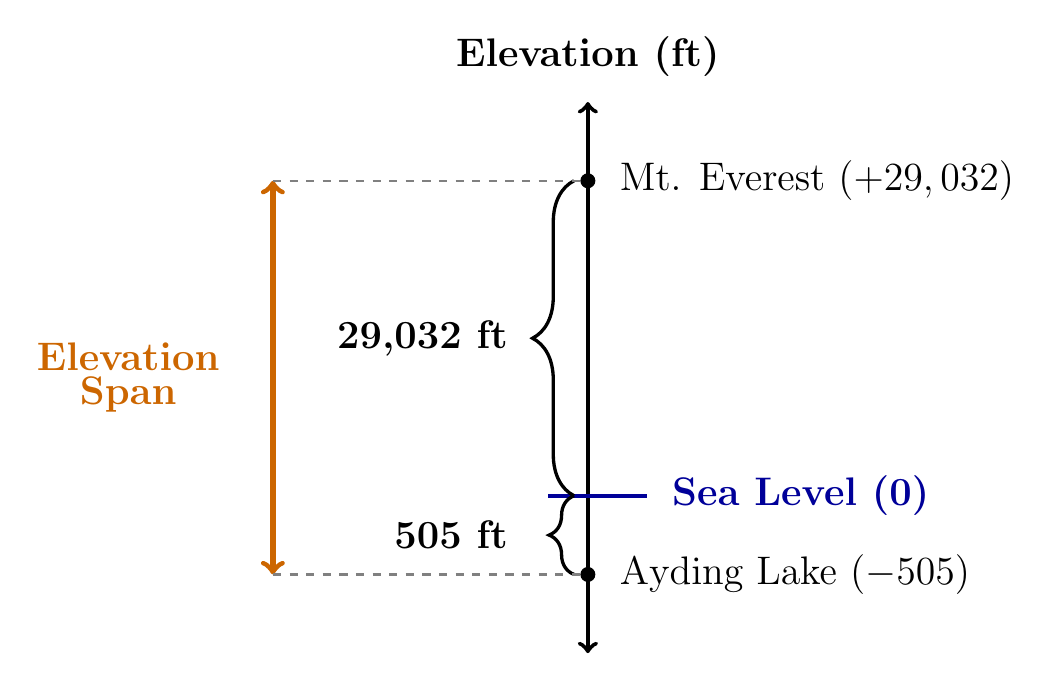
\begin{tikzpicture}[scale=0.5]  %China Elevation Span
    % Draw Vertical Axis
    \draw[ultra thick, <->] (0,-4) -- (0,10) node[above, yshift=5pt] {\textnormal{\Large\textbf{Elevation (ft)}}};

    % Sea Level Line
    \draw[blue!60!black, ultra thick] (-1,0) -- (1.5,0) node[right, xshift=5pt] {\textnormal{\Large\textbf{Sea Level (0)}}};

    % Mount Everest Point
    \filldraw[black] (0,8) circle (5pt) node[right, xshift=8pt] {\textnormal{\Large Mt. Everest ($+29,032$)}};

    % Ayding Lake Point
    \filldraw[black] (0,-2) circle (5pt) node[right, xshift=8pt] {\textnormal{\Large Ayding Lake ($-505$)}};

    % Braces
    \draw [decorate, decoration={brace, amplitude=9pt, raise=5pt}, very thick] (0,-2) -- (0,0)
        node [midway, left=25pt] {\textnormal{\Large\textbf{505 ft}}};

    \draw [decorate, decoration={brace, amplitude=15pt, raise=5pt}, very thick] (0,0) -- (0,8)
        node [midway, left=25pt] {\textnormal{\Large\textbf{29,032 ft}}};

    % Total Span Arrow - Stacked on two lines with fixed line break
    \draw[<->, orange!80!black, line width=2pt] (-8,-2) -- (-8,8)
        node [midway, left=15pt, align=center] {
            \Large \textbf{Elevation} \\
            \Large \textbf{Span}};

    % Guides
    \draw[dashed, gray, thick] (-8,8) -- (0,8);
    \draw[dashed, gray, thick] (-8,-2) -- (0,-2);
\end{tikzpicture}

\end{center}


%Alt Text
%Vertical number line showing topographic relief in China. Points are plotted at +29,032 (Mount Everest) and -505 (Ayding Lake). Braces indicate a distance of 29,032 units above zero and 505 units below zero. The total elevation span is shown as the combined vertical distance from -505 to +29,032

\begin{multipleChoice}
\choice{$29,032 - (-505) = -29,032 + (-505)$}
\choice{$29,032 - (-505) = 29,032 + (-505)$}
\choice{$29,032 - (-505) = -29,032 + 505$}
\choice[correct]{$29,032 - (-505) = 29,032 + 505$}
\end{multipleChoice}


\begin{problem}
Find the elevation span.  \textbf{Do not include commas in your answer}.

China's Elevation Span =  $\answer{29537}$ \ feet

\end{problem}
\end{problem}
\end{problem}

~ \\[2em]


\insightIcon{}

\section*{Extra Insight}

\normalsize
An \textbf{archipelagic nation} is a country made up of a group of islands and the surrounding water.
The Maldives is an archipelagic nation of over 1,000 islands located in the Indian Ocean. It is the lowest-lying country on Earth, with an average ground level elevation of less than 5 feet above sea level. It also has the world's smallest elevation span: just 16.7 feet above sea level. The islands are very flat!

\textbf{Highest Elevation:} 16.7 feet \textbf{above} sea level (Villingili Island)

\textbf{Lowest Elevation:} 0 feet, at sea level (Indian Ocean)


Scientists predict that most of the Maldives will be uninhabitable or completely submerged by the year 2100 if sea levels continue to rise at current rates.

\begin{center}
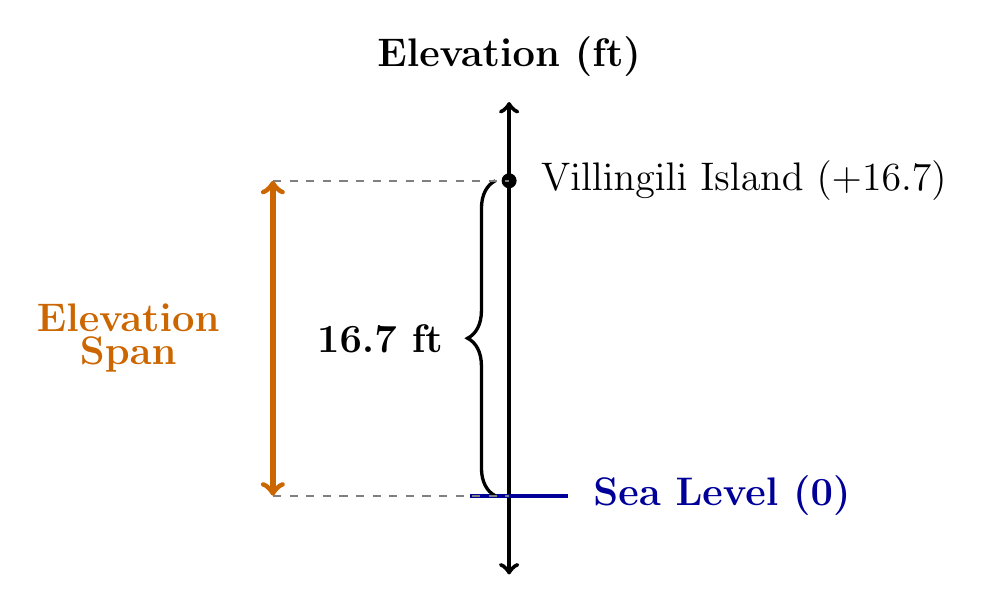
\begin{tikzpicture}[scale=0.5]
    % Draw Vertical Axis (Zoomed in scale)
    \draw[ultra thick, <->] (0,-2) -- (0,10) node[above, yshift=5pt] {\Large\textbf{Elevation (ft)}};

    % Current Sea Level Line
    \draw[blue!60!black, ultra thick] (-1,0) -- (1.5,0) node[right, xshift=5pt] {\Large\textbf{Sea Level (0)}};

    % Future Sea Level Projection (Dashed Line for 2100)
    %\draw[red, thick, dashed] (-1,4) -- (1.5,4) node[right, xshift=5pt, text=red] {\textbf{Predicted Level (2100)}};

    % Villingili Island Point (+16.7)
    % Note: On this scale, we'll place it at y=8 for visibility
    \filldraw[black] (0,8) circle (5pt) node[right, xshift=8pt] {\Large Villingili Island (+16.7)};

    % Braces
    \draw [decorate, decoration={brace, amplitude=10pt, raise=5pt}, very thick] (0,0) -- (0,8)
        node [midway, left=20pt] {\Large\textbf{16.7 ft}};

    % Total Span Arrow (Orange for accessibility)
    \draw[<->, orange!80!black, line width=2pt] (-6,0) -- (-6,8)
        node [midway, left=15pt, align=center] {\Large\textbf{Elevation}\\\Large\textbf{Span}};

    % Guides
    \draw[dashed, gray, thick] (-6,8) -- (0,8);
    \draw[dashed, gray, thick] (-6,0) -- (0,0);
\end{tikzpicture}
\end{center}



\end{document}